\documentclass[12pt]{ctexart}
\usepackage{amsfonts,amssymb}
\usepackage{float}
\usepackage{graphicx}
\usepackage{amsmath}
\usepackage{listings}
\usepackage{geometry}
\usepackage[usenames,dvipsnames]{xcolor}
\usepackage{setspace}
\geometry{a4paper}
\geometry{top=2cm} 
\geometry{bottom=2cm}
\geometry{left=0.5cm}
\geometry{right=1cm}

\title{微分方程数值解~项目作业 4}
\author{凌子恒 \\ 信息与计算科学 3200102551}

\begin{document}

\maketitle

\subsection*{理论分析}

\subsubsection*{热方程}

由 $h=\dfrac{1}{20}$ 及定义域为 $[0,1]$ 知 $x$ 方向上分成 $21$ 个点。

$\begin{cases}
	r=\dfrac{k\nu}{h^2}\\
	h=\dfrac{1}{20}\\
	\nu=1
\end{cases}\Rightarrow k=\dfrac{h^2}{\nu}r=\dfrac{r}{100}$。

尝试运用 $s$-stage RK method:

$\begin{cases}
	y^i=f(U^n+k\sum\limits_{l=1}^{s}a_{i,l}y^l,t_n+c_ik)\\
	U^{n+1}=U^n+k\sum\limits_{l=1}^s b_ly^l\\
	f(u,t)=u_t=\nu u_{xx}=\dfrac{\nu}{h^2}(u(x+h,t)-2u(x,t)+u(x-h,t))
\end{cases}\\
\Rightarrow\begin{cases}
	y^i_j=\dfrac{\nu}{h^2}(U^n_{j+1}-2U^n_j+U^n_{j-1}+k\sum\limits_{l=1}^sa_{i,l}(y^l_{j+1}-2y^l_j+y^l_{j-1}))\\
	U^{n+1}_j=U^n_j+k\sum\limits_{l=1}^s b_ly^l_j
\end{cases}$。

Gauss 消元法解得 $y$,代入即可。

\subsubsection*{平流方程}

欲求解 $([x_l,x_r],T)$ 的解,需要在更大的区间上取点,以保证所有贡献都被计算。

以 Lax-Friedrichs 为例,考虑转移方程,$T$ 每变化 $k$ 时 $x$ 至多变化 $h$,故需在包含 $[x_l-\dfrac{T}{k}h,x_r+\dfrac{T}{k}h]$ 的区间上取点。其余方法同理。

\subsection*{实现思路}

各方法的实现基于:

\begin{itemize}
	\item solution.h 中的 solution 类存放结果,其支持 operator()(x,t) 查询 $(x,t)$ 处拟合值。
	\item linear.h 中的两个线性方程组求解方法,分别是三对角矩阵和一般矩阵的求解。
\end{itemize}

\subsubsection*{热方程}

热方程的全部方法实现在 heat.h 中。

Crank-Nicolson,  BTCS, FTCS 方法名称分别为 CN, BTCS, FTCS,均基于同一个基类 theta\_method,即对于 (12.22) 的实现,再具体代入三种 $\theta$。

Example 11.258 和 Example 11.227 方法名称分别为 RKM2, GLRKM1,均基于同一个基类 RKM,其实现了一般的 $s$-stage RK method 在热方程中的应用。

\subsubsection*{平流方程}

平流方程的全部方法实现在 advection.h 中。

Lax-Friedrichs,  Lax-Wendroff, upwind, Beam-Warming 方法名称分别为 LF, LW, upwind, BW,均基于同一个基类 advection,其实现了所有只与上一层有关的、转移矩阵为循环矩阵的方法。

leapfrog 方法名称为 leapfrog,由于其需要之前两层的结果,故单独实现。其第二层的结果使用与 Lax-Friedrichs 一样的方程。

\subsection*{实验结果和结论分析}

\subsubsection*{热方程}

图如下:

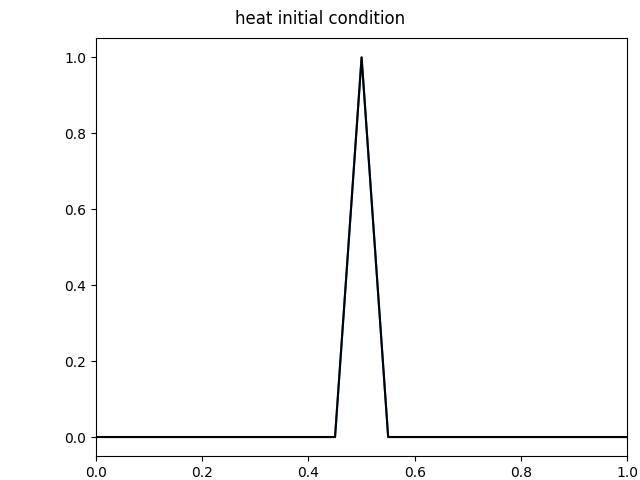
\includegraphics[scale=1.05]{heat initial condition.jpg}

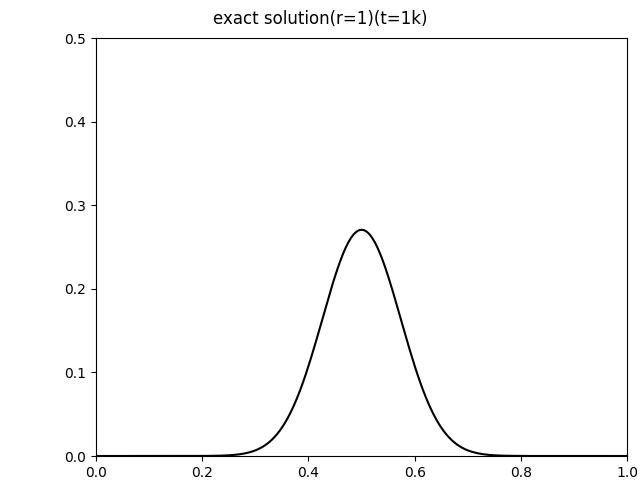
\includegraphics[scale=0.35]{exact solution(r=1)(t=1k).jpg}
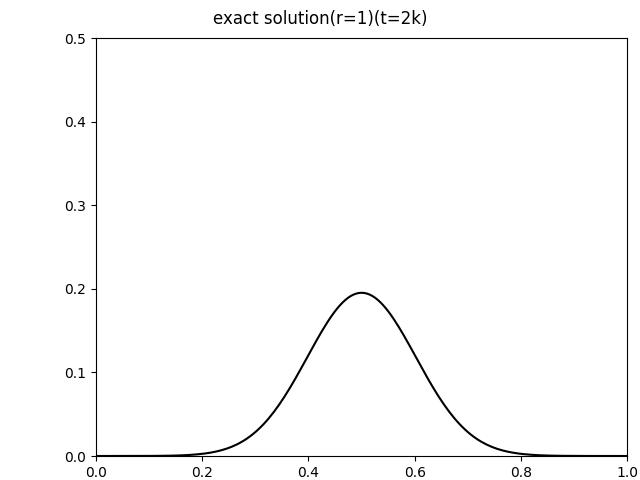
\includegraphics[scale=0.35]{exact solution(r=1)(t=2k).jpg}
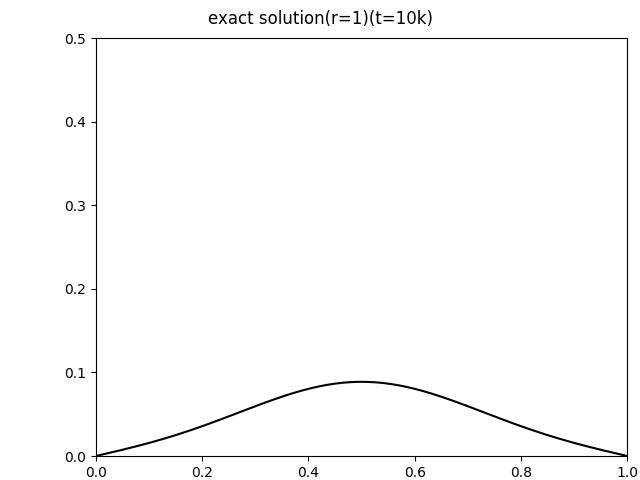
\includegraphics[scale=0.35]{exact solution(r=1)(t=10k).jpg}

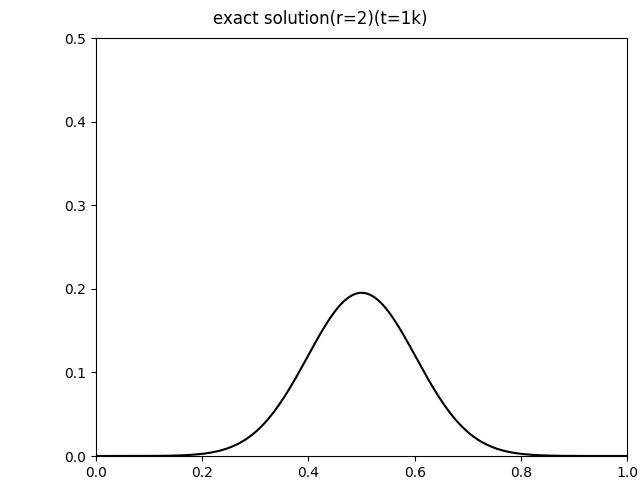
\includegraphics[scale=0.35]{exact solution(r=2)(t=1k).jpg}
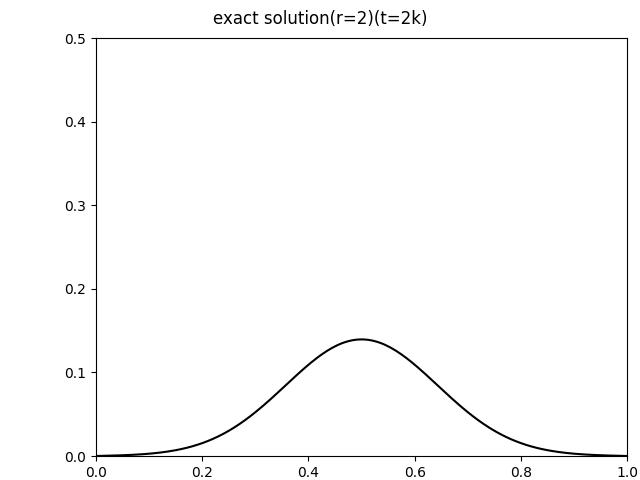
\includegraphics[scale=0.35]{exact solution(r=2)(t=2k).jpg}
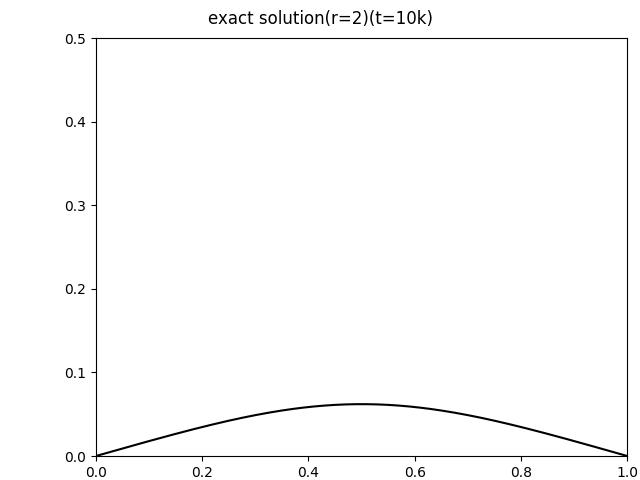
\includegraphics[scale=0.35]{exact solution(r=2)(t=10k).jpg}

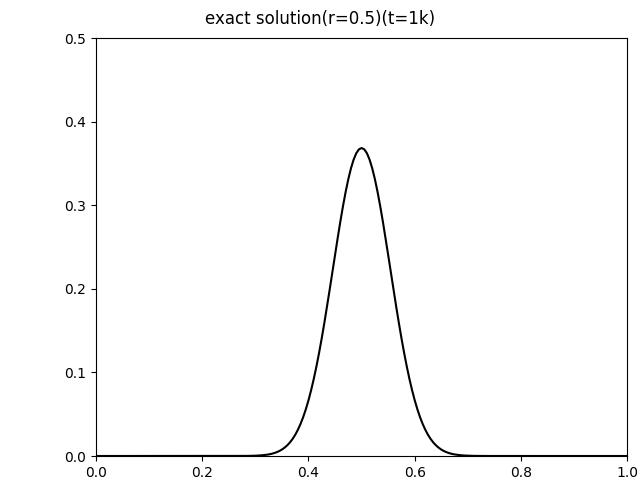
\includegraphics[scale=0.35]{exact solution(r=0.5)(t=1k).jpg}
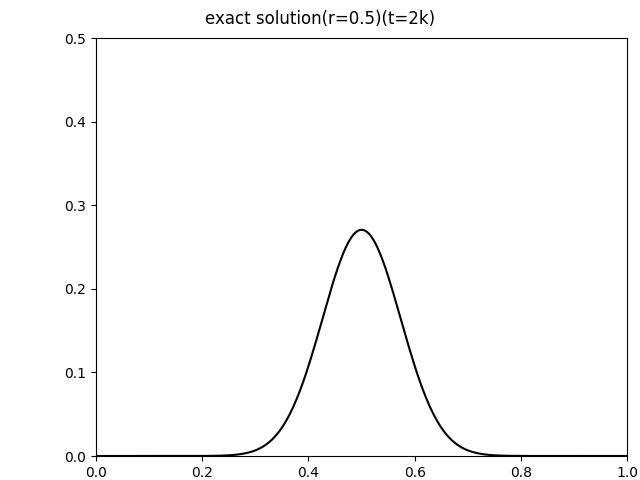
\includegraphics[scale=0.35]{exact solution(r=0.5)(t=2k).jpg}
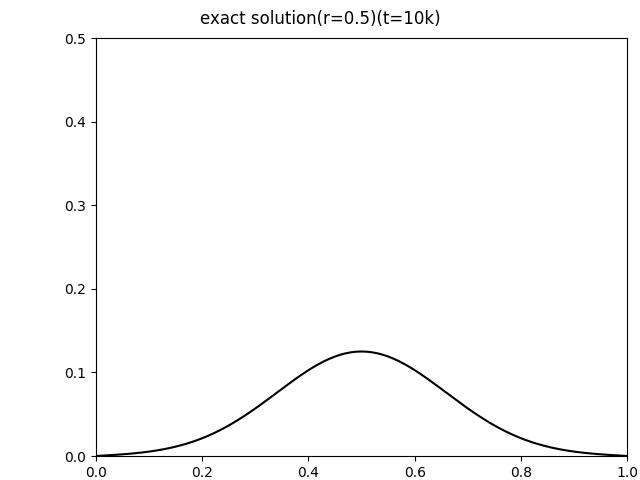
\includegraphics[scale=0.35]{exact solution(r=0.5)(t=10k).jpg}

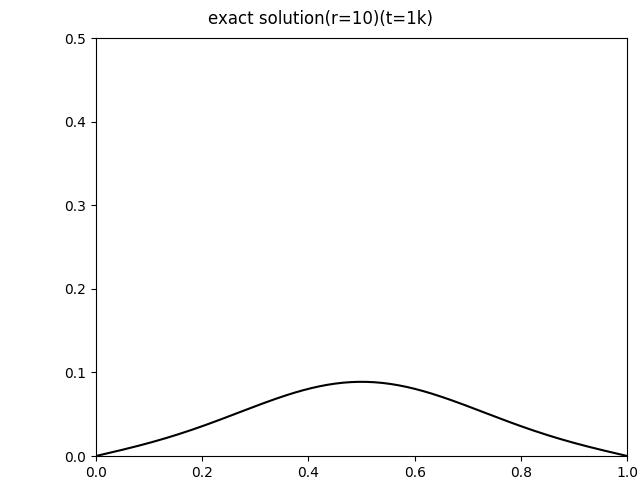
\includegraphics[scale=0.35]{exact solution(r=10)(t=1k).jpg}
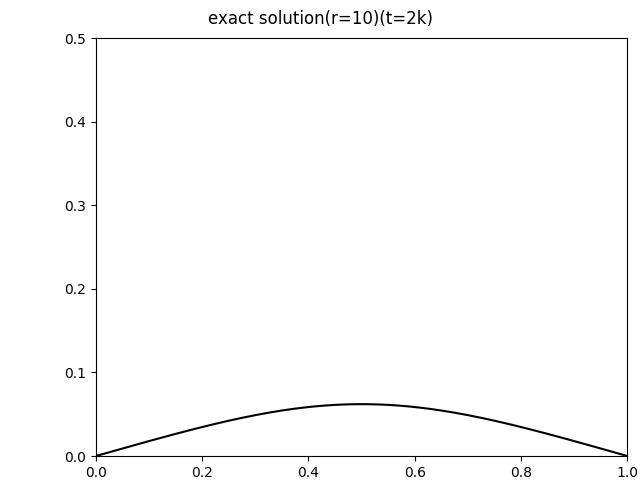
\includegraphics[scale=0.35]{exact solution(r=10)(t=2k).jpg}
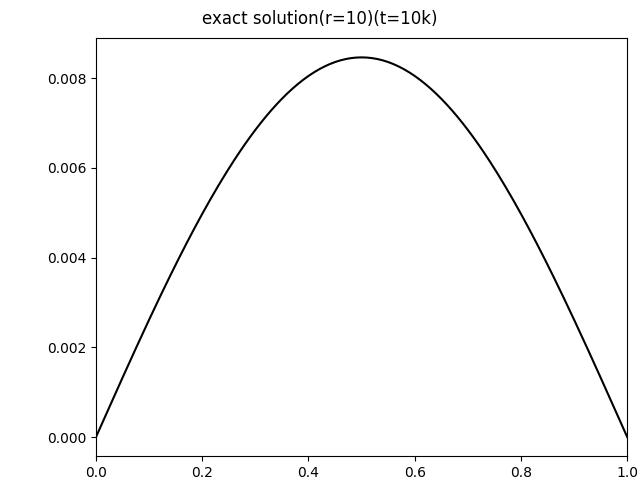
\includegraphics[scale=0.35]{exact solution(r=10)(t=10k).jpg}

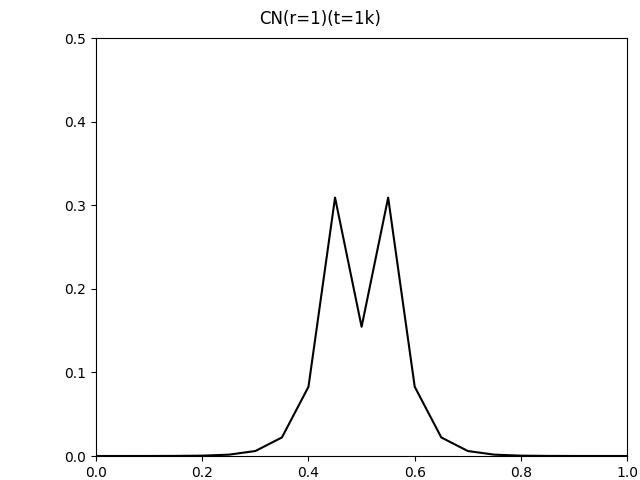
\includegraphics[scale=0.35]{CN(r=1)(t=1k).jpg}
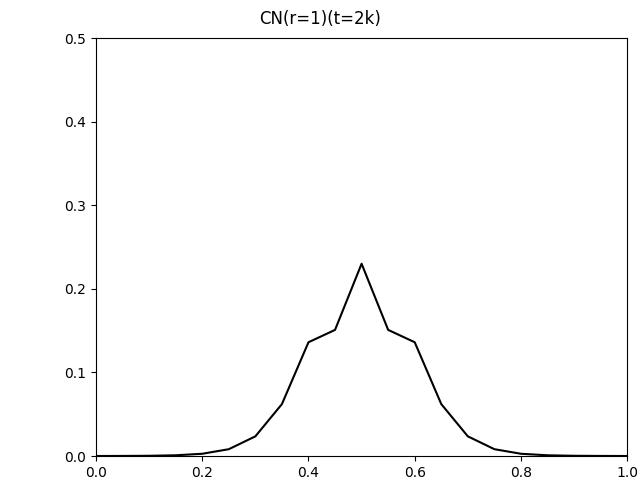
\includegraphics[scale=0.35]{CN(r=1)(t=2k).jpg}
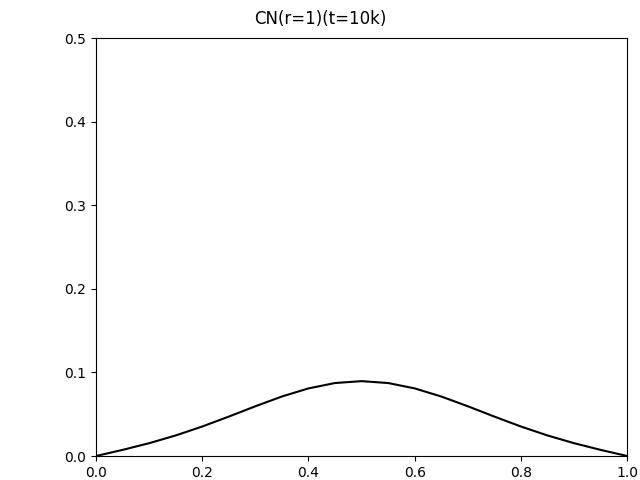
\includegraphics[scale=0.35]{CN(r=1)(t=10k).jpg}

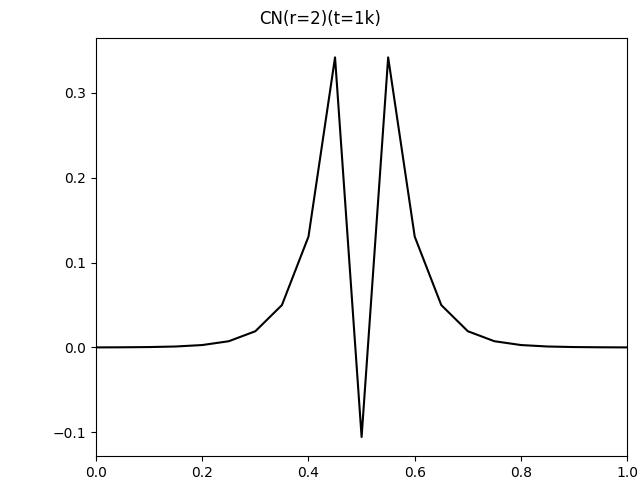
\includegraphics[scale=0.35]{CN(r=2)(t=1k).jpg}
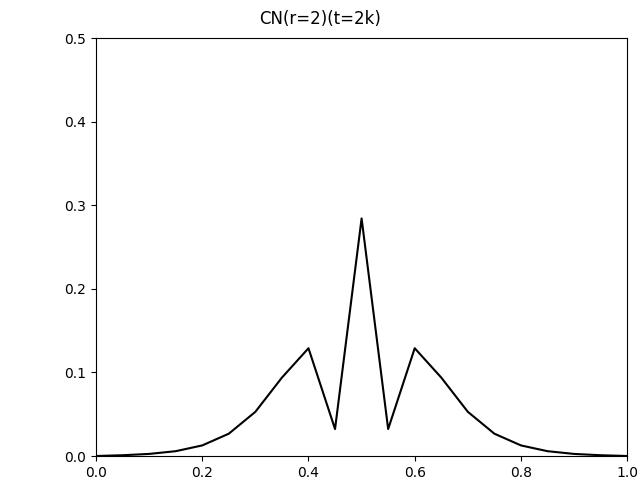
\includegraphics[scale=0.35]{CN(r=2)(t=2k).jpg}
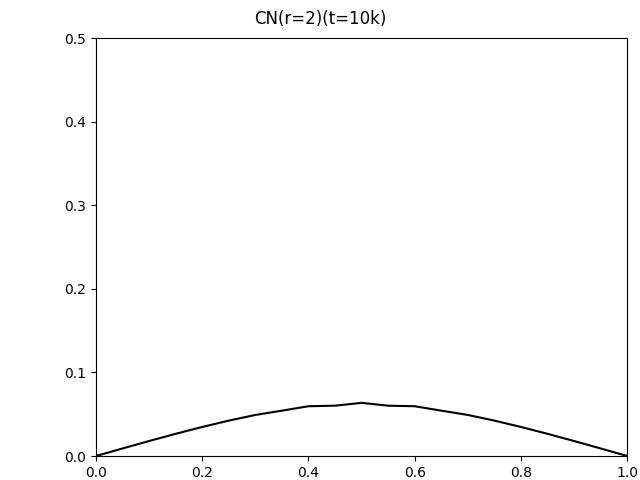
\includegraphics[scale=0.35]{CN(r=2)(t=10k).jpg}

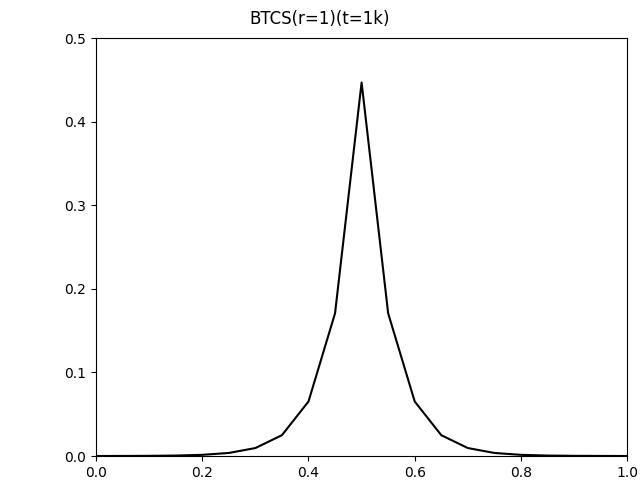
\includegraphics[scale=0.35]{BTCS(r=1)(t=1k).jpg}
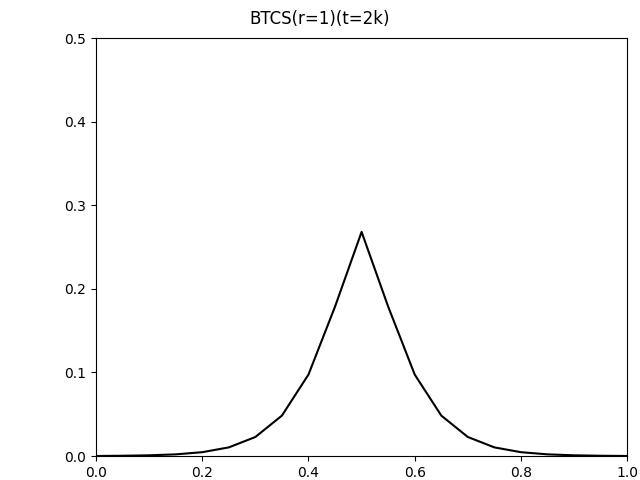
\includegraphics[scale=0.35]{BTCS(r=1)(t=2k).jpg}
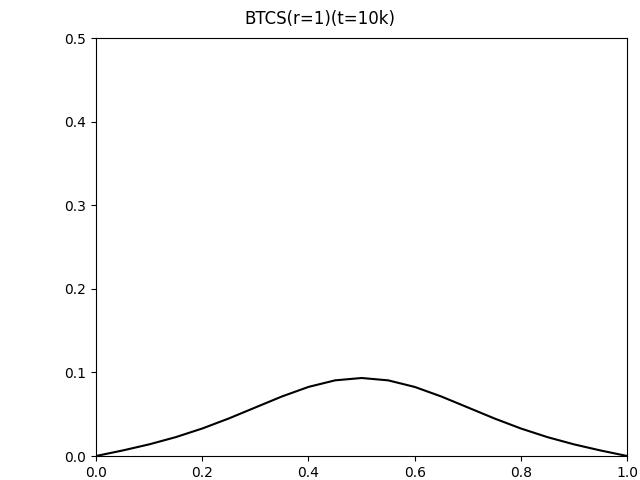
\includegraphics[scale=0.35]{BTCS(r=1)(t=10k).jpg}

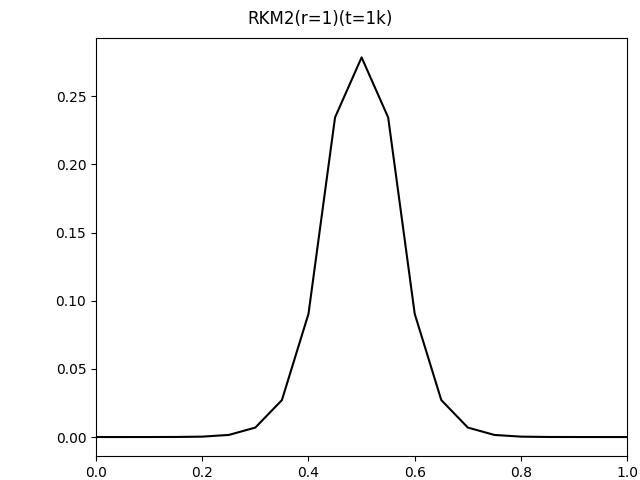
\includegraphics[scale=0.35]{RKM2(r=1)(t=1k).jpg}
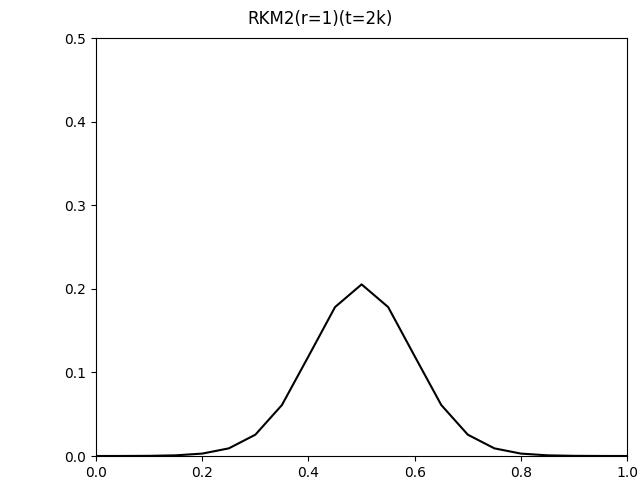
\includegraphics[scale=0.35]{RKM2(r=1)(t=2k).jpg}
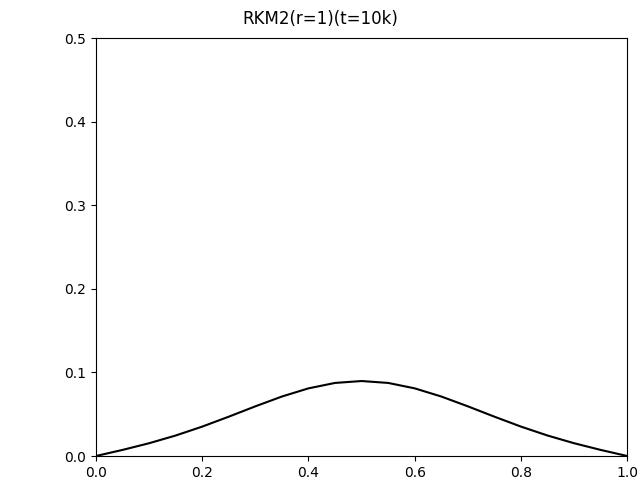
\includegraphics[scale=0.35]{RKM2(r=1)(t=10k).jpg}

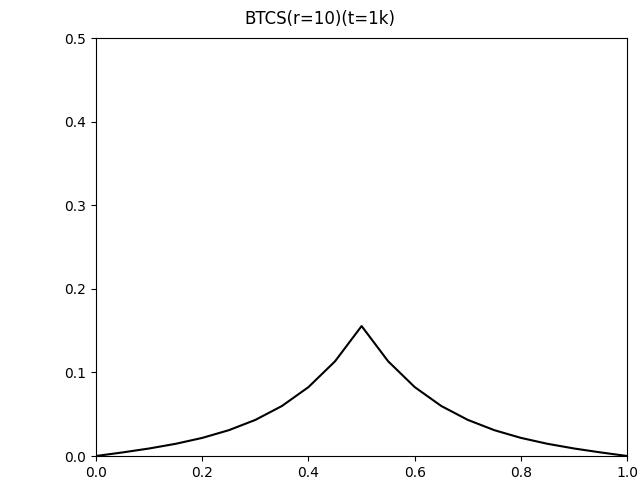
\includegraphics[scale=0.35]{BTCS(r=10)(t=1k).jpg}
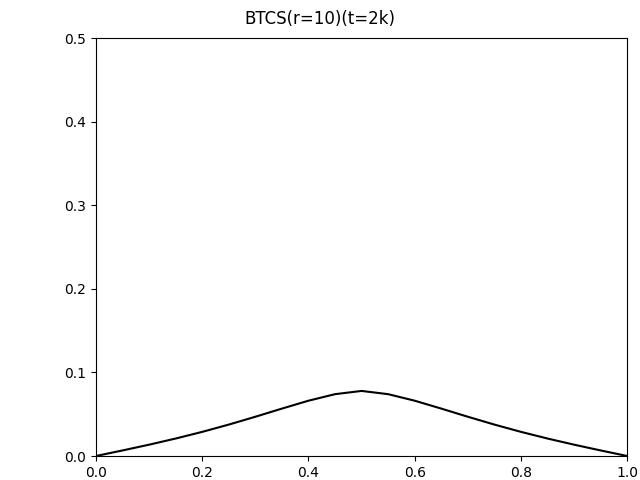
\includegraphics[scale=0.35]{BTCS(r=10)(t=2k).jpg}
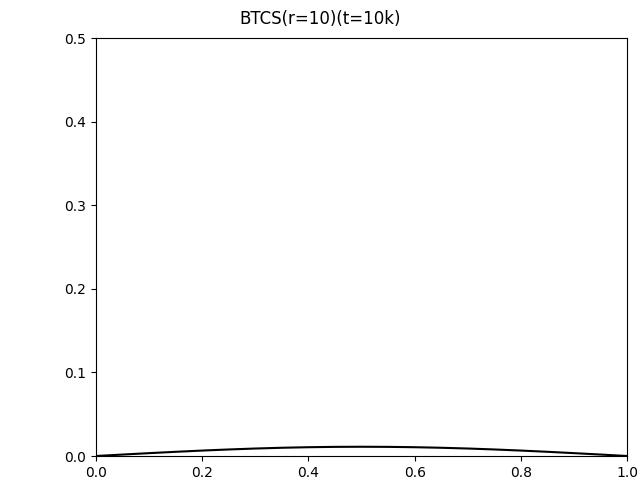
\includegraphics[scale=0.35]{BTCS(r=10)(t=10k).jpg}

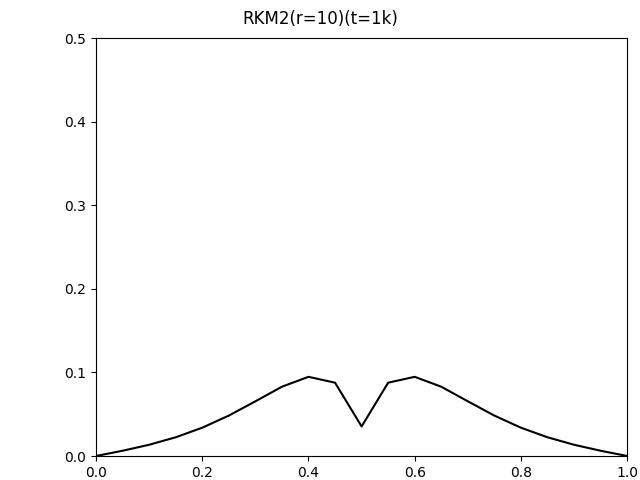
\includegraphics[scale=0.35]{RKM2(r=10)(t=1k).jpg}
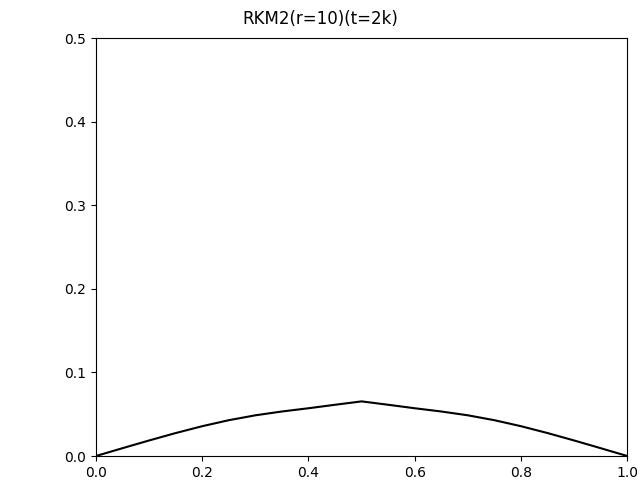
\includegraphics[scale=0.35]{RKM2(r=10)(t=2k).jpg}
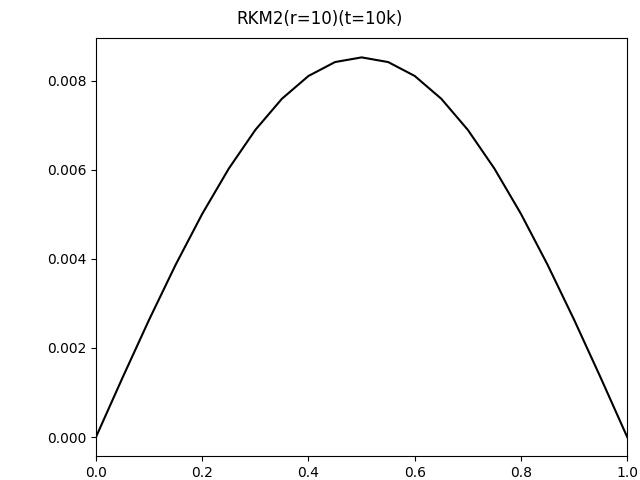
\includegraphics[scale=0.35]{RKM2(r=10)(t=10k).jpg}

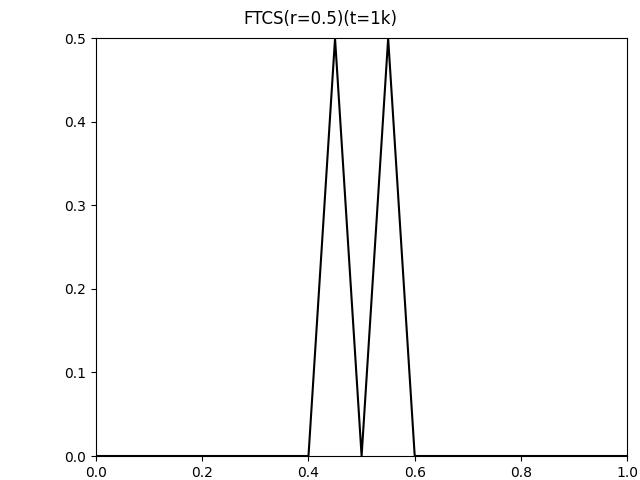
\includegraphics[scale=0.35]{FTCS(r=0.5)(t=1k).jpg}
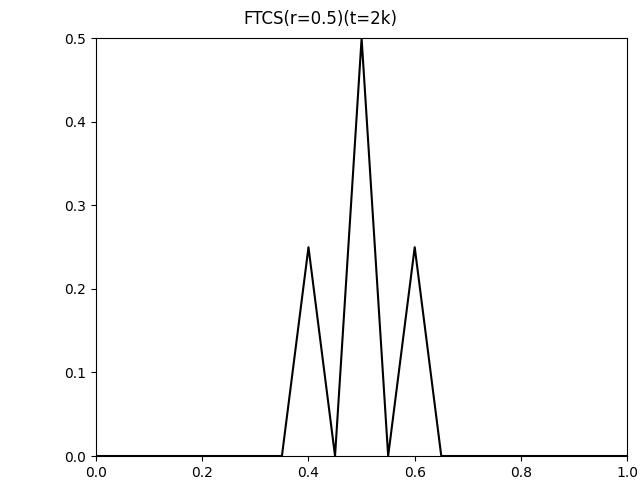
\includegraphics[scale=0.35]{FTCS(r=0.5)(t=2k).jpg}
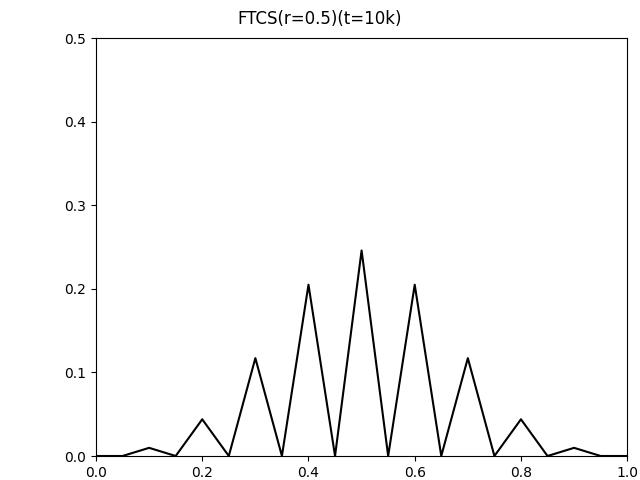
\includegraphics[scale=0.35]{FTCS(r=0.5)(t=10k).jpg}

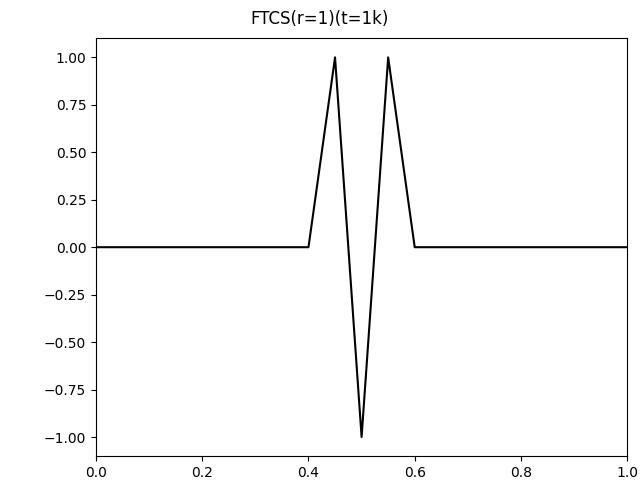
\includegraphics[scale=0.35]{FTCS(r=1)(t=1k).jpg}
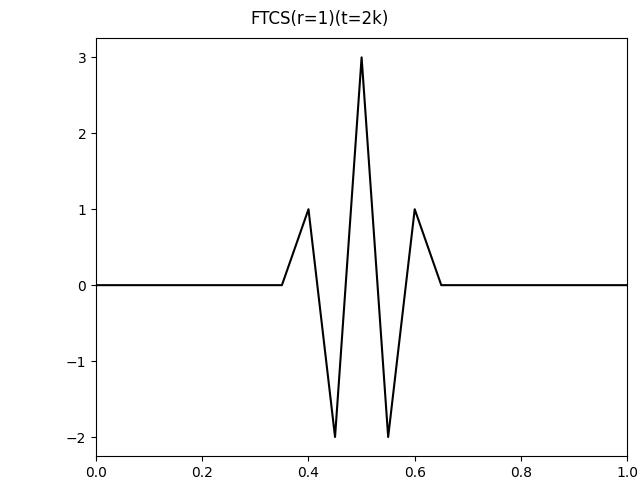
\includegraphics[scale=0.35]{FTCS(r=1)(t=2k).jpg}
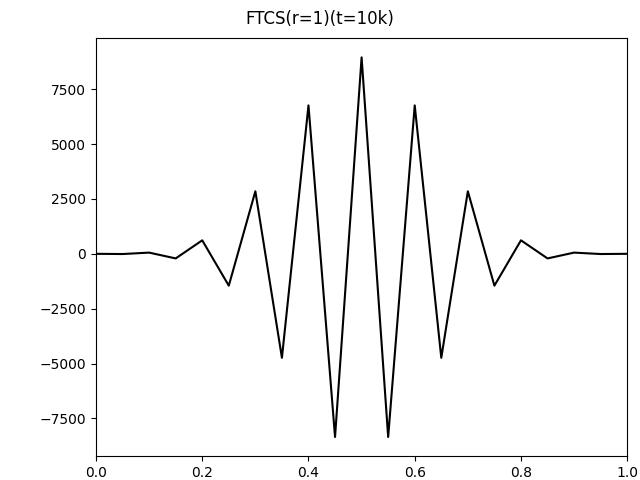
\includegraphics[scale=0.35]{FTCS(r=1)(t=10k).jpg}

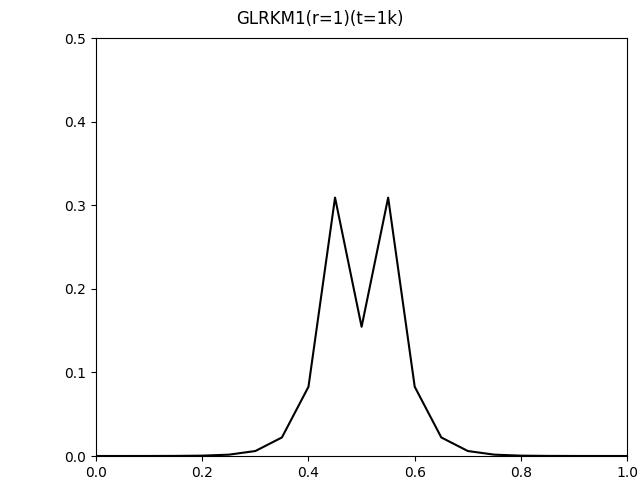
\includegraphics[scale=0.35]{GLRKM1(r=1)(t=1k).jpg}
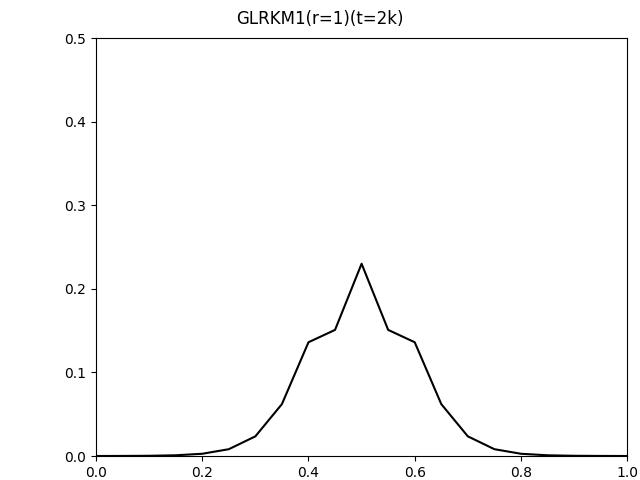
\includegraphics[scale=0.35]{GLRKM1(r=1)(t=2k).jpg}
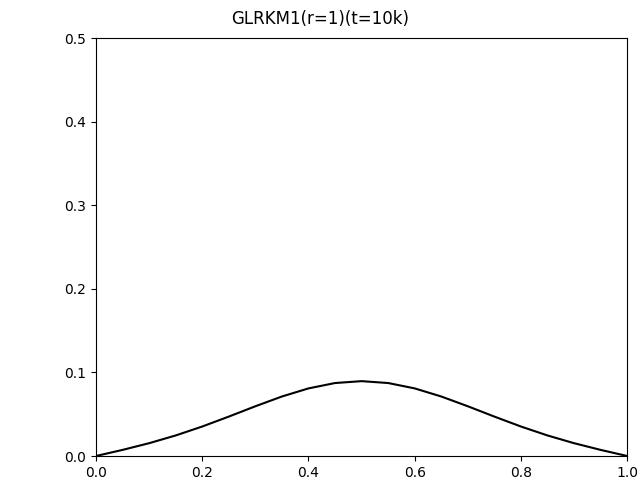
\includegraphics[scale=0.35]{GLRKM1(r=1)(t=10k).jpg}

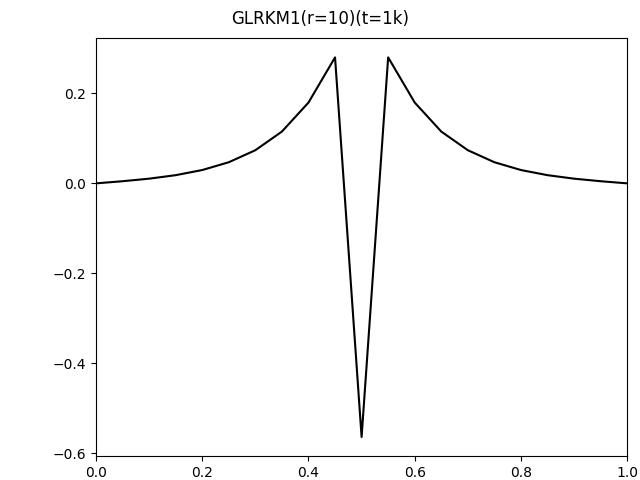
\includegraphics[scale=0.35]{GLRKM1(r=10)(t=1k).jpg}
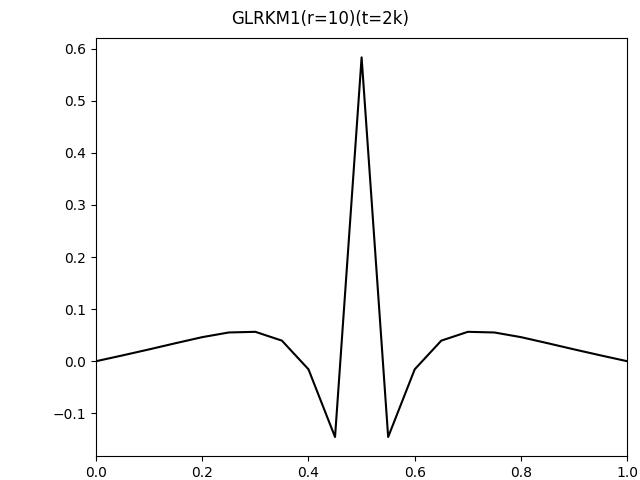
\includegraphics[scale=0.35]{GLRKM1(r=10)(t=2k).jpg}
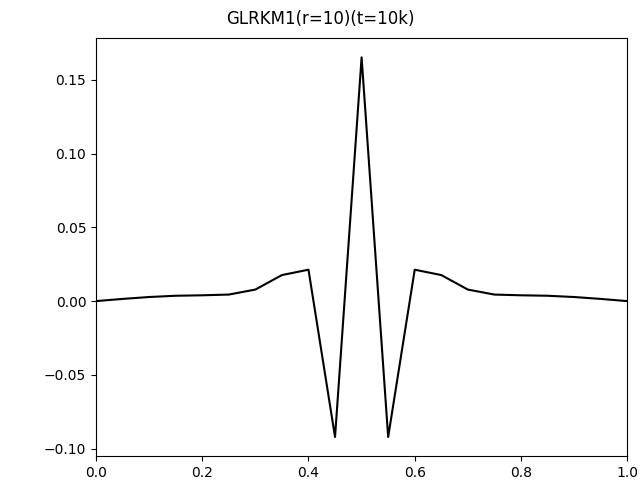
\includegraphics[scale=0.35]{GLRKM1(r=10)(t=10k).jpg}

从图像可以看出,Crank-Nicolson 方法 ($r=2,t=1k$),FTCS 方法 $(r=1)$,$1$-stage Gauss-Legendre RK 方法 ($r=10$) 的解都违反了极值原理。

各方法中,对于 $r=1$,Example 11.258 的拟合效果较好。

对于 $r=10$,各方法的表现都很差。

\subsubsection*{平流方程}

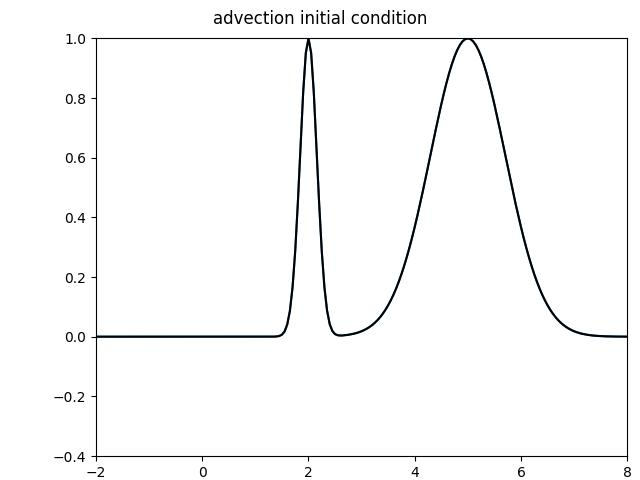
\includegraphics[scale=0.52]{advection initial condition.jpg}
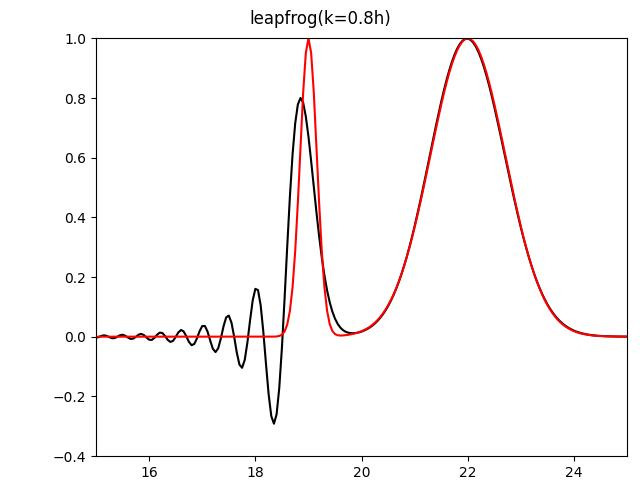
\includegraphics[scale=0.52]{leapfrog(k=0.8h).jpg}

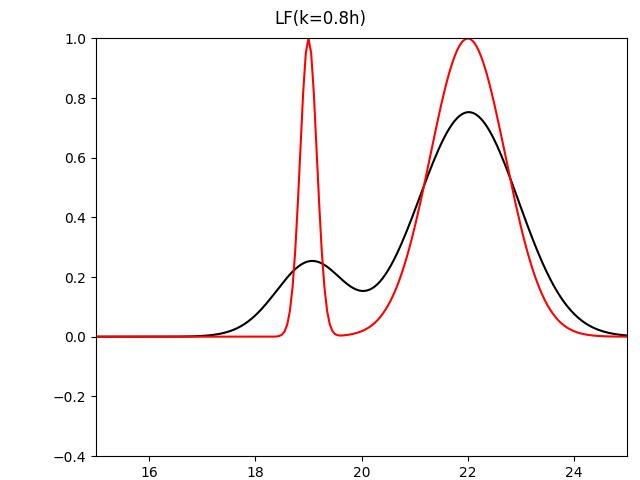
\includegraphics[scale=0.52]{LF(k=0.8h).jpg}
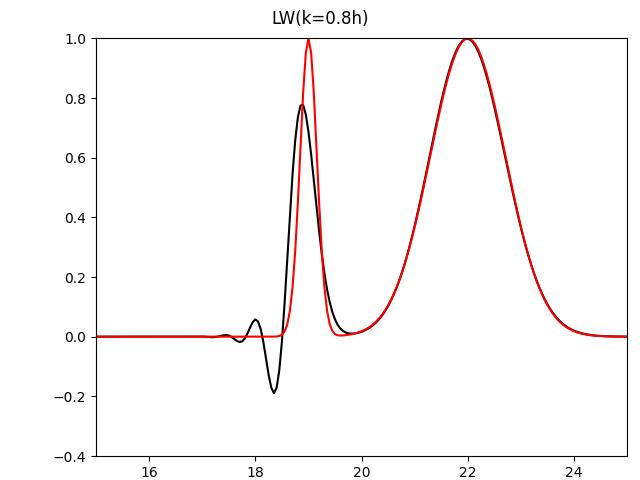
\includegraphics[scale=0.52]{LW(k=0.8h).jpg}

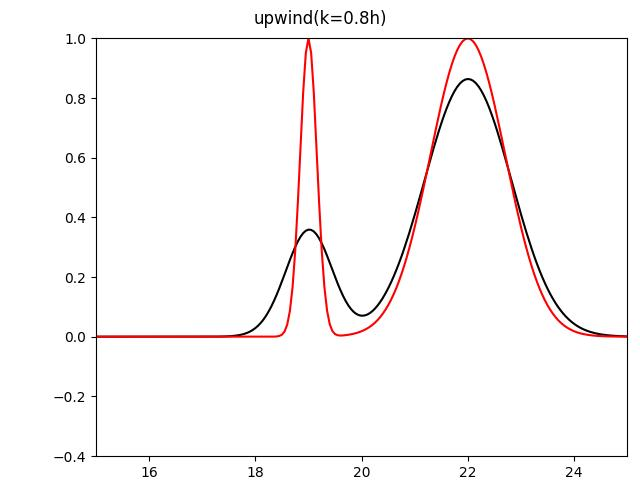
\includegraphics[scale=0.52]{upwind(k=0.8h).jpg}
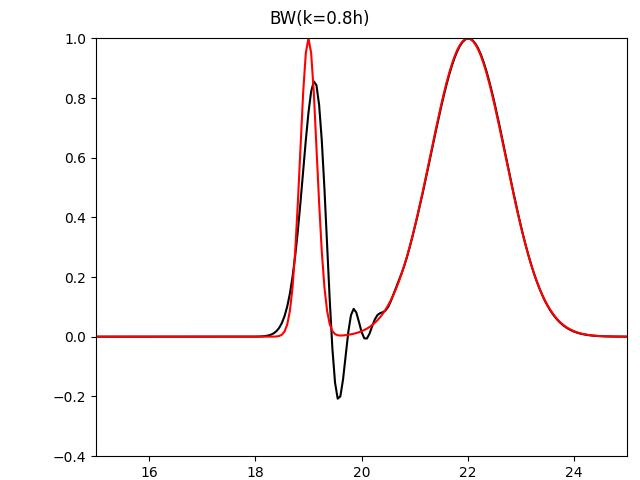
\includegraphics[scale=0.52]{BW(k=0.8h).jpg}

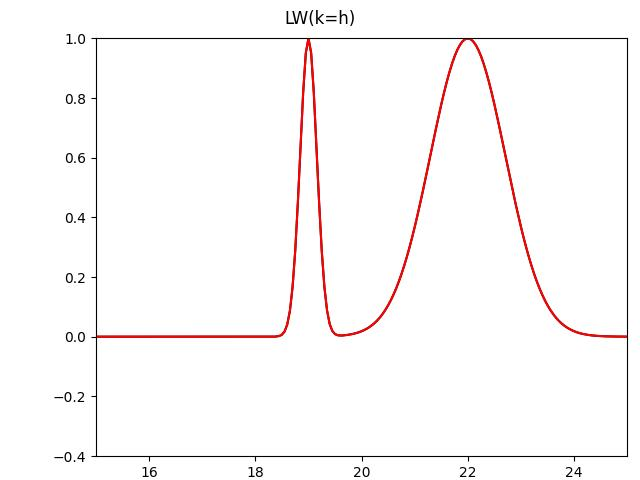
\includegraphics[scale=0.52]{LW(k=h).jpg}
\includegraphics[scale=0.52]{leapfrog(k=h).jpg}

\end{document}
